\section{Experiments}
\label{sec:experiments}

\subsection{Experimental setup}
\label{sec:experimental-setup}

\paragraph{Dataset and processing.}
We construct the dataset from 1,114 TCGA-BRCA H\&E slides. Tissue regions are divided into $512\times512$-pixel tiles, and CellViT++ is used to obtain nucleus contours, centroids, and predicted cell types. Tiles containing more than two predicted tumor nuclei are retained, producing approximately 1.4 million image tiles with aligned cellular maps and morphology/appearance vectors. Splits are defined at the patient level so that tiles from the same patient cannot occur in both training and evaluation. All generator fidelity results use held-out cases.

The cellular map contains separate channels for tumor, inflammatory, stromal, non-neoplastic epithelial, and necrotic cells. The morphology vector contains standardized summaries of nuclear geometry, gradient, and RGB appearance. Conditions, source images, generations, and cellular predictions are joined using the original tile identifier to prevent mismatches between experimental artifacts.

\paragraph{Generator.}
All experiments use the same 30,000-step CPathOGen checkpoint. No retraining, test-time fitting, or downstream-model information is used when generating the evaluation sets. Unless an intervention explicitly modifies a condition, its spatial map, morphology vector, diffusion seed, and generation parameters remain fixed. Fidelity-guided results use the eight-seed selection procedure described in Sec.~\ref{sec:fidelity-guidance}.

\paragraph{Cellular analyzers.}
CellViT++ is used during candidate selection and is therefore the in-loop analyzer. HoVer-Net and StarDist do not influence generation or selection and provide out-of-loop measurements. CellViT++ and HoVer-Net support nucleus segmentation and cell typing; StarDist provides segmentation without the corresponding five-class taxonomy. Results are therefore reported separately rather than treating the analyzers as interchangeable ground truth.

\paragraph{Downstream models and tasks.}
We evaluate ResNet-50, CTransPath, and UNI2-h as frozen feature extractors. Tile representations are mean-pooled within each patient and $\ell_2$-normalized. PAM50 is formulated as four-class prediction over Basal, HER2-enriched, Luminal A, and Luminal B subtypes. Class-balanced multinomial heads are evaluated using five patient-disjoint folds, with macro one-vs-rest AUC as the primary metric.

Overall survival remains censor-aware. Regularized Cox proportional-hazards heads are fitted after train-fold scaling and dimensionality reduction and evaluated using held-out Harrell's C-index. PathLUPI with CONCH is evaluated using its released breast-cancer survival model without refitting. Because the available data constitute a selected tile collection rather than each method's original whole-slide tiling pipeline, this result is an available-tile-bag transfer evaluation.

For counterfactual evaluation, one source tile in a patient's baseline bag is replaced by its generated variant. The resulting bag is evaluated with the patient's held-out prediction head. Counterfactuals are never used to train or select the downstream models.

\subsection{Distributional realism}
\label{sec:realism-experiment}

We measure distributional similarity using Fr\'echet Inception Distance (FID) and Kernel Inception Distance (KID). Both metrics use 2,000 generated images and the same held-out real reference set. The unfiltered evaluation contains one generation per condition. The fidelity-guided evaluation selects one image from eight candidates using only spatial agreement with the requested map. KID is reported as its raw mean and subset standard deviation.

\begin{table}[t]
\centering
\caption{Distributional realism on 2,000 held-out generations. The two generated rows use the same conditions, real reference set, and metric implementation.}
\label{tab:realism}
\setlength{\tabcolsep}{3.5pt}
\begin{tabular}{lcc}
\toprule
Evaluation set & FID $\downarrow$ & KID $\downarrow$ \\
\midrule
No seed filtering
    & 42.923
    & $0.02466\pm0.00340$ \\
CellViT++ selected
    & \textbf{36.717}
    & $\mathbf{0.01964\pm0.00332}$ \\
Real vs.\ real reference
    & 16.369
    & $0.00647$ \\
\bottomrule
\end{tabular}
\end{table}

As shown in Table~\ref{tab:realism}, fidelity-guided selection reduces FID from 42.923 to 36.717, an improvement of 6.206 points or 14.5\%. Mean KID decreases by 20.3\%. The improvement indicates that candidates agreeing more closely with the requested cellular map also tend to lie closer to the real-image distribution. The real-versus-real comparison provides a finite-sample reference rather than an attainable generator target.

We do not directly compare these values with FID or KID reported by generators evaluated on different datasets. Both metrics depend strongly on magnification, tile selection, sample count, reference-set composition, and feature-extractor implementation.

\subsection{Spatial fidelity}
\label{sec:spatial-fidelity-experiment}

Spatial fidelity asks whether the generated image expresses the cell abundance and locations specified by its input map. We evaluate $N=1{,}000$ fidelity-guided generations. For every tile, the input-map centroids are compared with nuclei recovered independently from the generated H\&E image.

Total-count fidelity is the Spearman correlation between the requested and recovered number of nuclei across images. Per-type count fidelity computes the same correlation separately for tumor, inflammatory, stromal, necrotic, and non-neoplastic epithelial cells and macro-averages the five values. Typed counts are not reported for StarDist.

Localization is measured using one-to-one Hungarian centroid matching at tolerances of 25 and 50 pixels. A match must also agree in cell type for CellViT++ and HoVer-Net; StarDist matching is position-only. Centroid precision and recall are combined into F1. As a negative control, each requested map is paired with a real tile from another patient. This control contains realistic nuclei but has no reason to reproduce the requested cellular arrangement.

\begin{table*}[t]
\centering
\caption{Spatial fidelity on $N=1{,}000$ selected images. Count columns are Spearman correlations with the input map. Centroid F1 uses one-to-one matching; typed analyzers additionally require cell-type agreement.}
\label{tab:spatial}
\setlength{\tabcolsep}{7pt}
\begin{tabular}{lcccc}
\toprule
Method
& Total count $\rho\uparrow$
& Per-type count $\rho\uparrow$
& Centroid F1 @ 25 px $\uparrow$
& Centroid F1 @ 50 px $\uparrow$ \\
\midrule
CellViT++
& \textbf{0.952}
& \textbf{0.612}
& 0.726
& 0.773 \\
HoVer-Net
& 0.908
& 0.525
& 0.625
& 0.668 \\
StarDist
& 0.928
& N/A
& \textbf{0.798}
& \textbf{0.831} \\
Random real tile
& $-0.031$
& $-0.020$
& 0.134
& 0.255 \\
\bottomrule
\end{tabular}
\end{table*}

\begin{figure}[t]
\centering
\scriptsize
\setlength{\tabcolsep}{1pt}

\begin{tabular}{@{}ccc@{}}
\textbf{Cell map} & \textbf{Real H\&E} & \textbf{Generated H\&E} \\[-1pt]

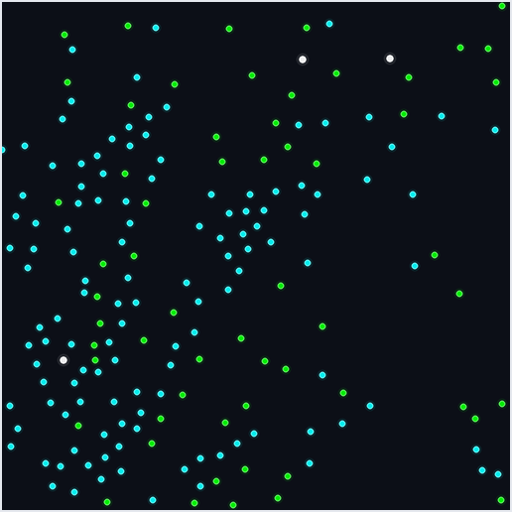
\includegraphics[width=0.31\columnwidth]
{00_baseline_assets/foundational__TCGA-A2-A0CW_x65536_y47104_TL__seed_0000029256/paper_map.png}
&
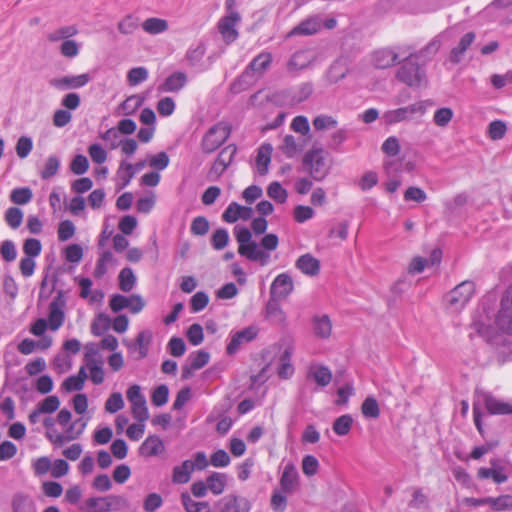
\includegraphics[width=0.31\columnwidth]
{00_baseline_assets/foundational__TCGA-A2-A0CW_x65536_y47104_TL__seed_0000029256/source_real.png}
&
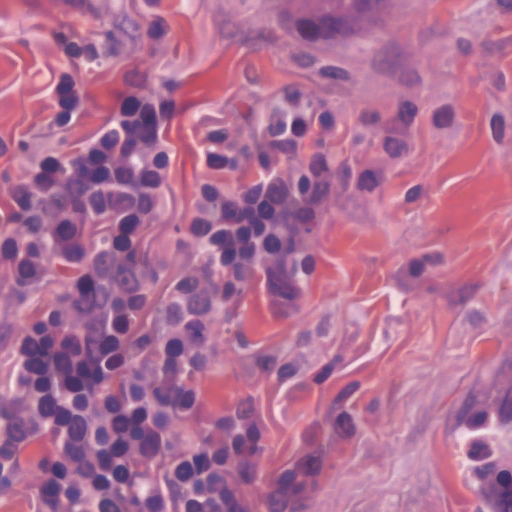
\includegraphics[width=0.31\columnwidth]
{00_baseline_assets/foundational__TCGA-A2-A0CW_x65536_y47104_TL__seed_0000029256/generated.png}
\\[1pt]

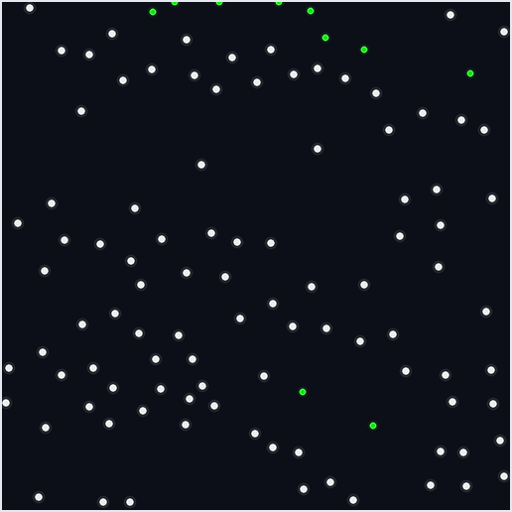
\includegraphics[width=0.31\columnwidth]
{00_baseline_assets/foundational__TCGA-A8-A083_x14336_y30720_BR__seed_0000032098/paper_map.png}
&
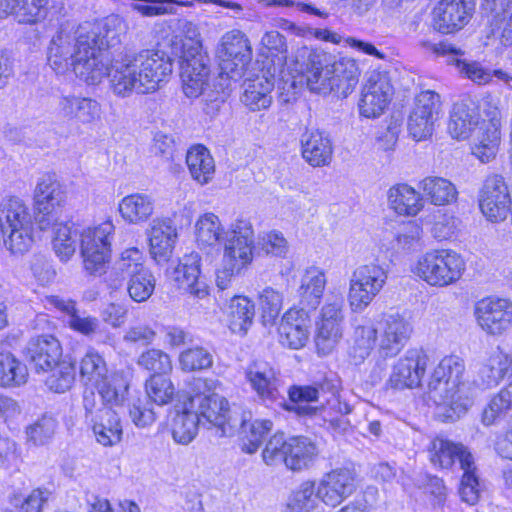
\includegraphics[width=0.31\columnwidth]
{00_baseline_assets/foundational__TCGA-A8-A083_x14336_y30720_BR__seed_0000032098/source_real.png}
&
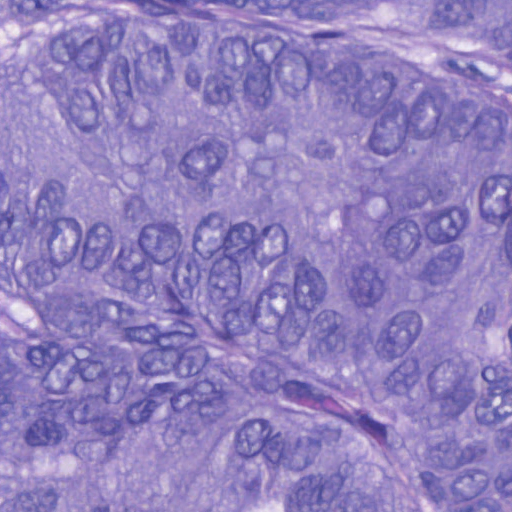
\includegraphics[width=0.31\columnwidth]
{00_baseline_assets/foundational__TCGA-A8-A083_x14336_y30720_BR__seed_0000032098/generated.png}
\\[1pt]

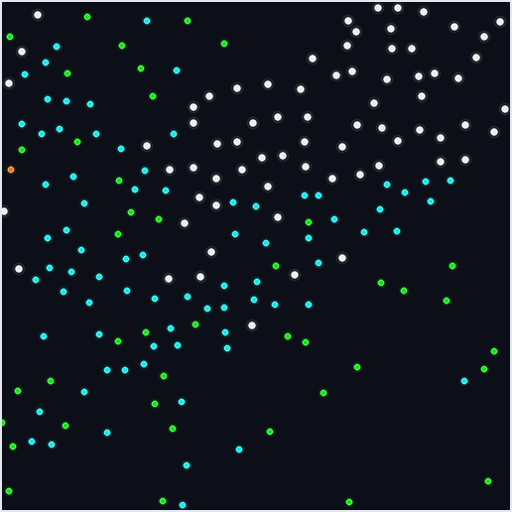
\includegraphics[width=0.31\columnwidth]
{00_baseline_assets/035__TCGA-AR-A5QQ_x40960_y31744_BL__seed_1404673085/paper_map.png}
&
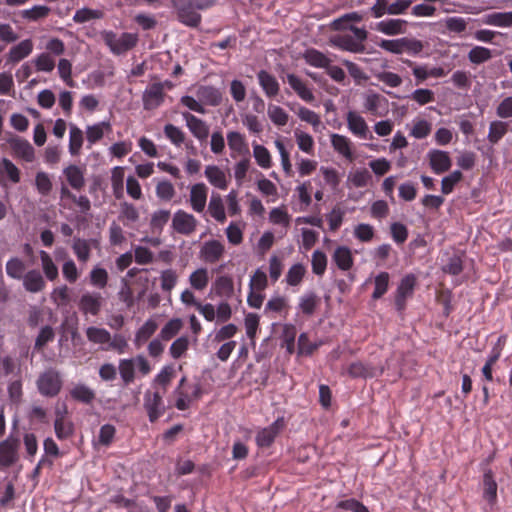
\includegraphics[width=0.31\columnwidth]
{00_baseline_assets/035__TCGA-AR-A5QQ_x40960_y31744_BL__seed_1404673085/source_real.png}
&
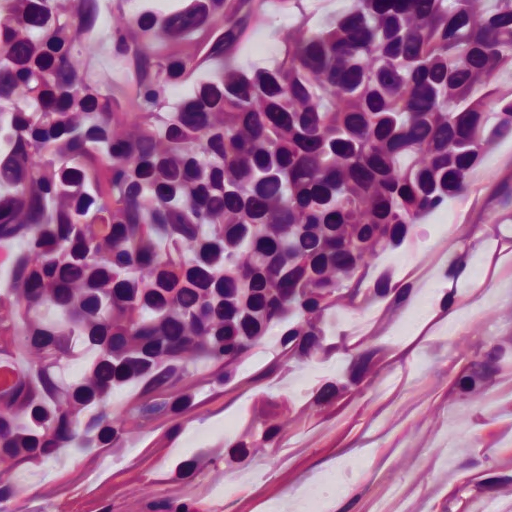
\includegraphics[width=0.31\columnwidth]
{00_baseline_assets/035__TCGA-AR-A5QQ_x40960_y31744_BL__seed_1404673085/generated.png}
\\
\end{tabular}

\par\vspace{2pt}
\begingroup
\definecolor{mapcyan}{RGB}{0,255,255}
\definecolor{mapgreen}{RGB}{0,255,0}
\definecolor{mapyellow}{RGB}{255,255,0}
\definecolor{maporange}{RGB}{255,128,0}
\setlength{\fboxsep}{0pt}

\newcommand{\mapkey}[2]{%
  \raisebox{-0.25ex}{%
    \fcolorbox{black}{#1}{%
      \rule{0pt}{1.05ex}\rule{1.05ex}{0pt}%
    }%
  }\,#2%
}

\mapkey{white}{Tumor}\quad
\mapkey{mapcyan}{Immune}\quad
\mapkey{mapgreen}{Stroma}\\[-1pt]
\mapkey{mapyellow}{Dead}\quad
\mapkey{maporange}{Non-neoplastic epithelium}
\endgroup

\caption{Representative spatial conditions and their corresponding H\&E tiles. Each row shows the requested cellular map, the associated real tile, and a generated tile conditioned on the same map. Generated images reproduce the broad cellular composition and organization while remaining distinct from the real reference.}
\label{fig:spatial_grid}
\end{figure}


Table~\ref{tab:spatial} shows strong total-count recovery for all three analyzers: $\rho=0.952$ for CellViT++, 0.908 for HoVer-Net, and 0.928 for StarDist. The near-zero random-tile correlation demonstrates that the result is specific to the requested map rather than a general tendency to detect plausible numbers of nuclei in H\&E tissue.

Per-type recovery is more difficult because it requires both successful synthesis and agreement between cellular taxonomies. Nevertheless, CellViT++ and HoVer-Net retain correlations of 0.612 and 0.525. At 50 pixels, typed centroid F1 reaches 0.773 for CellViT++ and 0.668 for HoVer-Net. StarDist obtains 0.831 without requiring type agreement and should therefore not be interpreted as outperforming the typed analyzers. Representative input maps, real tiles, and generated tiles are shown in Figure~\ref{fig:spatial_grid}.

\subsection{Morphology and appearance fidelity}
\label{sec:morphology-fidelity-experiment}

Morphology fidelity is evaluated from two complementary perspectives. The across-image analysis asks whether natural differences among requested conditions are preserved in generated images. For $N=1{,}000$ selected generations, each input feature is correlated with the corresponding value recovered from the generated image.

The within-image analysis tests intervention fidelity more directly. For 200 source conditions, each of seven controls is varied over
$\{-1,-0.5,0,+0.5,+1\}$ standard deviations while retaining the spatial map, non-target morphology entries, and diffusion seed. This produces
$200\times7\times5=7{,}000$ controlled images. Spearman correlation is computed across the five doses for each source, and the table reports the median source-level correlation. Figure~\ref{fig:morphology_grid} uses the wider $\{-2,-1,0,+1,+2\}$ range for qualitative visualization.

Nuclear size, eccentricity, and solidity are recovered from predicted contours. Gradient and RGB values are measured within the detected nuclear regions. Perimeter remains part of the generator condition but is omitted from the compact table because of its strong relationship with nuclear area. Macro $\rho$ is the unweighted mean of the seven displayed features.

\begin{table*}[t]
\centering
\caption{Morphology fidelity. Across-image rows use $N=1{,}000$ selected images. Controlled rows report median within-source Spearman correlation over five same-seed doses for 200 sources.}
\label{tab:morphology}
\small
\begin{tabular*}{\textwidth}{@{\extracolsep{\fill}}lcccccccc@{}}
\toprule
Method
& Size
& Eccentricity
& Solidity
& Gradient
& Red
& Green
& Blue
& Macro \\
& $\rho\uparrow$
& $\rho\uparrow$
& $\rho\uparrow$
& $\rho\uparrow$
& $\rho\uparrow$
& $\rho\uparrow$
& $\rho\uparrow$
& $\rho\uparrow$ \\
\midrule
Across images CellViT++
& \textbf{0.941}
& \textbf{0.820}
& \textbf{0.649}
& 0.878
& \textbf{0.951}
& \textbf{0.961}
& \textbf{0.928}
& \textbf{0.876} \\
Across images HoVer-Net
& 0.896
& 0.798
& 0.499
& 0.886
& 0.942
& 0.958
& 0.925
& 0.843 \\
Across images StarDist
& 0.935
& 0.760
& 0.570
& \textbf{0.892}
& 0.950
& 0.954
& \textbf{0.928}
& 0.855 \\
\midrule
Controlled CellViT++
& \textbf{1.000}
& \textbf{1.000}
& \textbf{0.900}
& \textbf{1.000}
& \textbf{1.000}
& \textbf{1.000}
& \textbf{1.000}
& \textbf{0.986} \\
Controlled HoVer-Net
& \textbf{1.000}
& \textbf{1.000}
& \textbf{0.900}
& \textbf{1.000}
& \textbf{1.000}
& \textbf{1.000}
& \textbf{1.000}
& \textbf{0.986} \\
Controlled StarDist
& \textbf{1.000}
& \textbf{1.000}
& 0.500
& \textbf{1.000}
& \textbf{1.000}
& \textbf{1.000}
& \textbf{1.000}
& 0.929 \\
\bottomrule
\end{tabular*}
\end{table*}

\begin{figure*}[t]
\centering
\scriptsize
\setlength{\tabcolsep}{1pt}
\renewcommand{\arraystretch}{0.98}

\newcommand{\morphtile}[2]{%
  \includegraphics[width=\linewidth]
  {01_morphology_controls/#1/#2.png}%
}

\begin{tabular}{@{}
  >{\raggedleft\arraybackslash}m{0.075\textwidth}
  *{7}{>{\centering\arraybackslash}m{0.125\textwidth}}
  @{}}

& Nuclear size
& Eccentricity
& Solidity
& Gradient
& Red
& Green
& Blue \\

$-2$ SD
& \morphtile{nuclear_size}{minus_2sd}
& \morphtile{eccentricity}{minus_2sd}
& \morphtile{solidity}{minus_2sd}
& \morphtile{gradient}{minus_2sd}
& \morphtile{red}{minus_2sd}
& \morphtile{green}{minus_2sd}
& \morphtile{blue}{minus_2sd}
\\[1pt]

$-1$ SD
& \morphtile{nuclear_size}{minus_1sd}
& \morphtile{eccentricity}{minus_1sd}
& \morphtile{solidity}{minus_1sd}
& \morphtile{gradient}{minus_1sd}
& \morphtile{red}{minus_1sd}
& \morphtile{green}{minus_1sd}
& \morphtile{blue}{minus_1sd}
\\[1pt]

$0$ SD
& \morphtile{nuclear_size}{zero_sd}
& \morphtile{eccentricity}{zero_sd}
& \morphtile{solidity}{zero_sd}
& \morphtile{gradient}{zero_sd}
& \morphtile{red}{zero_sd}
& \morphtile{green}{zero_sd}
& \morphtile{blue}{zero_sd}
\\[1pt]

$+1$ SD
& \morphtile{nuclear_size}{plus_1sd}
& \morphtile{eccentricity}{plus_1sd}
& \morphtile{solidity}{plus_1sd}
& \morphtile{gradient}{plus_1sd}
& \morphtile{red}{plus_1sd}
& \morphtile{green}{plus_1sd}
& \morphtile{blue}{plus_1sd}
\\[1pt]

$+2$ SD
& \morphtile{nuclear_size}{plus_2sd}
& \morphtile{eccentricity}{plus_2sd}
& \morphtile{solidity}{plus_2sd}
& \morphtile{gradient}{plus_2sd}
& \morphtile{red}{plus_2sd}
& \morphtile{green}{plus_2sd}
& \morphtile{blue}{plus_2sd}
\\
\end{tabular}

\caption{Controlled morphology and appearance interventions for one representative H\&E condition. Each column varies one feature over five standardized levels while preserving the spatial map, non-target controls, and diffusion seed. The wider visual sweep complements the central five-level sweep used for quantitative within-image correlations.}
\label{fig:morphology_grid}
\end{figure*}

Across images, macro correlation reaches 0.876 for CellViT++, 0.843 for HoVer-Net, and 0.855 for StarDist. Nuclear size and RGB appearance are particularly consistent across analyzers. Solidity is the weakest feature, especially for HoVer-Net, reflecting its sensitivity to small differences in predicted nuclear boundaries.

Within-image correlations increase to 0.986 for CellViT++ and HoVer-Net and 0.929 for StarDist. Values of 1.0 indicate correct monotonic ordering across the five requested doses, not exact calibration of the generated morphology. The lower StarDist solidity correlation again localizes the primary disagreement to contour shape rather than color or size.

\subsection{Counterfactual model probing}
\label{sec:counterfactual-probing}

\paragraph{Interventions.}
We construct five intervention families, each designed to isolate a different property of the input tile:

\begin{itemize}
    \item \textbf{Stain brightness} jointly shifts the mean red, green, and blue controls while preserving channel variance, spatial structure, and nuclear geometry. It serves as the principal appearance-related nuisance intervention.
    \item \textbf{Nuclear enlargement} increases mean nuclear area and perimeter together while preserving their variance and all non-target controls.
    \item \textbf{Nuclear shape irregularity} increases eccentricity and perimeter while decreasing solidity, with nuclear area held fixed.
    \item \textbf{Peritumoral immune burden} adds 80, 160, or 320 inflammatory centroids around the tumor support while retaining the tumor channel, other cell types, morphology vector, and diffusion seed.
    \item \textbf{Tumor--immune separation} relocates the existing inflammatory centroids from maximal mixing through low, intermediate, and high separation to maximal segregation. Tumor coordinates and tumor and immune cell counts remain fixed.
\end{itemize}

For stain and morphology, the primary analysis compares a generated 0-SD reference with $+0.5$, $+1$, and $+1.5$ SD variants. The peritumoral experiment uses $+80$ immune cells as its reference and compares it with $+160$ and $+320$. The separation experiment uses maximal mixing as its reference and compares it with the four progressively separated patterns. Thus, the spatial measurements represent movement along a controlled spatial trajectory rather than a comparison with an unmodified real image.

Every intervention cohort begins from 1,000 baseline tiles. A baseline tile is the statistical unit; multiple dose levels belonging to that tile do not increase $N$. Effects are first averaged across the target variants of each tile and subsequently averaged across tiles.

\paragraph{Response metrics.}
For a $C$-class PAM50 model, let
$p_i^{(0)}$ and $p_i^{(\delta)}$ denote the baseline and intervention probability vectors for tile $i$. We measure output displacement using total variation distance:
\begin{equation}
D_{\mathrm{TV},i}
=
\frac{1}{2}
\sum_{c=1}^{C}
\left|
p_{ic}^{(\delta)}-p_{ic}^{(0)}
\right|.
\label{eq:experiment-tvd}
\end{equation}
Prediction flip rate is the proportion of tiles for which the highest-probability PAM50 class changes.

For the trained survival models, TVD is calculated from the five-year survival distribution
$[S(5),1-S(5)]$, and a flip denotes crossing the $S(5)=0.5$ threshold. PathLUPI does not expose a directly comparable calibrated five-year probability; its TVD and flip rate use the final released discrete-survival bin. Its absolute intervention values should therefore be interpreted within PathLUPI rather than directly against the native five-year survival heads.

We introduce the Biology-to-Nuisance Ratio (BNR) to contrast sensitivity to biological interventions with sensitivity to stain brightness. Let
\begin{equation}
D_{\mathrm{morph}}
=
\frac{
D_{\mathrm{enlarge}}+D_{\mathrm{shape}}
}{2},
\qquad
D_{\mathrm{spatial}}
=
\frac{
D_{\mathrm{immune}}+D_{\mathrm{separation}}
}{2}.
\end{equation}
The ratio is
\begin{equation}
\mathrm{BNR}
=
\frac{
\left(D_{\mathrm{morph}}+D_{\mathrm{spatial}}\right)/2
}{
D_{\mathrm{stain}}
}.
\label{eq:bnr}
\end{equation}
BNR greater than one indicates that biological morphology and spatial interventions produce larger probability changes, on average, than the matched stain nuisance intervention. BNR measures relative sensitivity and is not itself a predictive-performance score.

\begin{table*}[t]
\centering
\caption{Predictive performance and counterfactual response across downstream tasks. Intervention entries report mean TVD / prediction-flip rate. PAM50 performance is macro one-vs-rest AUC; survival performance is Harrell's C-index.}
\label{tab:xai_all_tasks}
\small
\renewcommand{\arraystretch}{1.30}
\setlength{\tabcolsep}{4.5pt}
\begin{adjustbox}{max width=\textwidth}
\begin{tabular}{lccccccc}
\toprule
\textbf{Model}
& \textbf{Performance}
& \shortstack{\textbf{Stain}\\\textbf{brightness}}
& \shortstack{\textbf{Nuclear}\\\textbf{enlargement}}
& \shortstack{\textbf{Shape}\\\textbf{irregularity}}
& \shortstack{\textbf{Immune}\\\textbf{burden}}
& \shortstack{\textbf{Tumor--immune}\\\textbf{separation}}
& \textbf{BNR} \\
\midrule

\multicolumn{8}{l}{
\textbf{PAM50 classification}
\hfill
\textit{Performance: macro AUC}
} \\
\midrule

ResNet-50
& 0.7627
& 0.0243 / 0.0238
& 0.0257 / 0.0281
& 0.0270 / 0.0241
& 0.0442 / 0.0626
& 0.0275 / 0.0267
& 1.2776 \\

CTransPath
& 0.8143
& 0.0104 / 0.0158
& 0.0093 / 0.0081
& 0.0094 / 0.0030
& 0.0152 / 0.0189
& 0.0105 / 0.0075
& 1.0694 \\

UNI2-h
& \textbf{0.8713}
& 0.0060 / 0.0094
& 0.0066 / 0.0115
& 0.0065 / 0.0073
& 0.0107 / 0.0137
& 0.0065 / 0.0065
& 1.2680 \\

\midrule
\multicolumn{8}{l}{
\textbf{Overall survival}
\hfill
\textit{Performance: C-index}
} \\
\midrule

ResNet-50
& 0.5445
& 0.0026 / 0.0024
& 0.0025 / 0.0017
& 0.0033 / 0.0003
& 0.0039 / 0.0000
& 0.0029 / 0.0005
& 1.1893 \\

CTransPath
& \textbf{0.6216}
& 0.0017 / 0.0014
& 0.0017 / 0.0017
& 0.0018 / 0.0000
& 0.0026 / 0.0005
& 0.0015 / 0.0010
& 1.1398 \\

UNI2-h
& 0.6209
& 0.0014 / 0.0021
& 0.0015 / 0.0021
& 0.0014 / 0.0010
& 0.0023 / 0.0021
& 0.0014 / 0.0003
& 1.1711 \\

PathLUPI + CONCH
& 0.5860
& 0.0043 / 0.0057
& 0.0049 / 0.0032
& 0.0043 / 0.0043
& 0.0207 / 0.0207
& 0.0036 / 0.0043
& 1.9488 \\

\bottomrule
\end{tabular}
\end{adjustbox}
\end{table*}

\paragraph{Counterfactual results.}
For PAM50, UNI2-h achieves the highest predictive performance with macro AUC 0.8713, followed by CTransPath at 0.8143 and ResNet-50 at 0.7627. Absolute intervention sensitivity differs substantially across models: ResNet-50 exhibits the largest probability movement, whereas UNI2-h is comparatively stable. This distinction illustrates why predictive performance and counterfactual sensitivity should be reported separately.

Peritumoral immune burden produces the largest PAM50 response for every model, reaching TVD 0.0442 and flip rate 0.0626 for ResNet-50. All PAM50 BNR values exceed one, although CTransPath is closest to parity at 1.0694. UNI2-h combines the smallest absolute output changes with BNR 1.2680, indicating that low overall sensitivity does not necessarily imply preferential invariance to biological controls.

CTransPath and UNI2-h achieve similar survival discrimination, with C-indices of 0.6216 and 0.6209. Survival TVDs and flip rates are smaller than their PAM50 counterparts because each counterfactual replaces only one tile within a patient-level bag. These values therefore measure the marginal effect of one controlled tile and should not be interpreted as standalone tile-classifier sensitivity.

PathLUPI shows the strongest response to peritumoral immune burden, with TVD and flip rate both equal to 0.0207, and the largest BNR at 1.9488. Across all survival models, BNR remains above one. Collectively, the results indicate that the evaluated models respond more strongly to controlled morphology and tumor--immune organization than to the matched stain-brightness intervention, while differing substantially in their absolute sensitivity and in which biological intervention produces the largest response.
